% This is LLNCS.DEM the demonstration file of
% the LaTeX macro package from Springer-Verlag
% for Lecture Notes in Computer Science,
% version 2.4 for LaTeX2e as of 16. April 2010
%
\documentclass[citenumber]{elsarticle}
\newtheorem{proposition}{Proposition}
\newtheorem{definition}{Definition}
\newtheorem{proof}{Proof}
\newtheorem{corollary}{Corollary}

\usepackage{hyperref}				% enlaces en el pdf
\hypersetup{colorlinks=true,        % colores en vez de cajas en los enlaces
			linkcolor=blue,         % color of internal links (change box color with linkbordercolor)
    		citecolor=blue,         % color of links to bibliography
    		filecolor=blue,         % color of file links
    		urlcolor=blue}          % color of external links	    

\usepackage{algorithm,algpseudocode}
\usepackage{multicol}
\usepackage{graphicx}           	% para manejar imagenes
\usepackage[utf8]{inputenc}
\usepackage{pstricks,pst-node,pst-tree} % Para la taxonomía
\usepackage{stackengine}				% Para listar los articulos en el nodo de la taxonomía
%\usepackage[table]{xcolor}			% Colores en el cronograma
%\usepackage{algorithm}				% Para el seudocódigo
%\usepackage{setspace}				% Para el seudocódigo
%\usepackage{amsmath}					% Para el seudocódigo
%\usepackage[noend]{algpseudocode}	% Para el seudocódigo
%\usepackage{multicol}				% Para el seudocódigo
%\usepackage{algorithmic}
\usepackage{tikz}
\usetikzlibrary{arrows}

\tikzset{
  treenode/.style = {align=center, inner sep=0pt, text centered,
    font=\sffamily},
%  circ/.style = {treenode, circle, white, font=\sffamily\bfseries, draw=black,
%    fill=black, text width=1.5em},% arbre rouge noir, noeud noir
  circ/.style = {treenode, circle, black, draw=black, 
    text width=1.5em, very thick},% arbre rouge noir, noeud rouge
  disc/.style = {treenode, circle, draw=gray,fill=gray,
    minimum width=1.5em, very thick}% arbre rouge noir, nil
}

\renewcommand{\algorithmicrequire}{\textbf{Input:}}
\renewcommand{\algorithmicensure}{\textbf{Output:}}

%-------------------------------------------------------------------------
% Configuring Taxonomy
%-------------------------------------------------------------------------
\setstackEOL{\\}
\def\psedge{\ncangles[angleA=-90,angleB=90]}
\psset{levelsep=20mm,treesep=1cm,nodesep=3pt, arrows=->}
\def\PSBL#1{\small\pspicture(7,0.5)\psTextFrame[shadow,
  fillstyle=solid,linecolor=blue,framearc=0.3](0,0)(7,0.5){%
    \shortstack{#1}}\endpspicture}
\def\PSBS#1{\pspicture(2.2,.5)\psTextFrame[shadow,
  fillstyle=solid,linecolor=blue,framearc=0.3](0,0)(2.2,0.5){%
    \shortstack{#1}}\endpspicture}

%-------------------------------------------------------------------------
% Referencias a una palabra
%-------------------------------------------------------------------------
\newcommand{\setword}[2]{%
  \phantomsection
  #1\def\@currentlabel{\unexpanded{#1}}\label{#2}%
}

\usepackage[margin=2.5cm]{geometry}	% Change margins

\begin{document}
%\mainmatter              % start of the contributions
%
\title{A parallel implementation of the fast--BR algorithm for reduct computation}

	\author[inaoe,uc]{Vad\'{\i}mir~Rodr\'{\i}guez-Diez\corref{cor1}}
	\ead{vladimir.rodriguez@inaoep.mx}
	\address[inaoe]{Computer Science Department\\
					Instituto Nacional de Astrof\'{\i}sica, \'{O}ptica y Electr\'{o}nica\\
					Luis Enrique Erro \# 1, Santa Mar\'{\i}a Tonantzintla, Puebla, 72840, M\'{e}xico} 
	\address[uc]{Electrical Engineering Department\\
				 Universidad de Camag\"{u}ey\\
				 Circv. Nte. km 5$\frac{1}{2}$, Camag\"{u}ey, Cuba}

%
\begin{abstract}
%
	Rough set theory is a relatively new mathematical theory to deal with imperfect knowledge, in particular with vague concepts. One of the key concepts within rough set theory is the concept of reduct. A reduct is a reduced set of attributes for the description of an dataset without changing its discernibility relations. The main limitation of rough set reducts is that computing the complete set of reducts of a dataset has exponential complexity regarding the number of attributes. Several attempts have been made to speed up reduct computation but most of these solutions looks for a subset of reducts.  This research proposal aims to develop a parallel implementation of the fast--BR algorithm, which is one of the fastest algorithms reported in the literature for computing all reducts of a dataset.
%
\end{abstract}
%
	\maketitle
%
\section{Introduction}
%
	Rough set theory (RST), proposed by Z. Pawlak in 1982 \cite{Pawlak81}, is a relatively new mathematical theory to deal with imperfect knowledge, in particular with vague concepts. Into RST, datasets are tables of objects (rows) described by a set of attributes (columns). When data is collected or recorded, every single aspect (attribute) of the object under study is considered to have a complete representation and to ensure that no potentially useful information is lost. As a result, datasets are usually characterized by a large number of attributes,  degrading the performance of machine learning tools \cite{Parthalain08}. One of the main concepts in RST is the notion of reduct, which is a minimal subset of attributes preserving the discernibility capacity of the whole set of attributes \cite{Pawlak91}. However, the main restriction of RST is that computing all reducts of a dataset has exponential complexity \cite{Skowron92}. Therefore, the development of fast algorithms for reduct computation is an active research line.
  
	Several attempts to speed up the reduct computation have been reported. Many of these algorithms are based on some heuristics. Another explored way to speed up reduct computation is parallelization \cite{Strakowski08}. There are also interesting alternatives such as the use of a parallel version of genetic algorithms \cite{Wroblewski98} and the transformation of the reduct computation problem to the well known SAT problem \cite{Jensen14}.
	
	RST reducts have been related to Typical Testors (TT) from the logical combinatorial approach to pattern recognition \cite{Chikalov2013}. Testor Theory was originally created by Cheguis and Yablonskii \cite{Cheguis55} as a tool for analysis of problems connected with control and diagnosis of faults in circuits. However, Testor Theory has been extended in order to be used for feature selection as shown in \cite{Dmitriev1966,Martinez01,Ruiz08}. Algorithms for typical testor computation can be applied to reduct computation due to the similarity between these two concepts \cite{Lazo15}. For this reason, we will treat algorithms for computing typical testors as reduct computation algorithms.
	
	The complete set of reducts of a dataset is useful for solving some practical problems and real--world applications. In \cite{Xu2013} a multi-objective cost-sensitive attribute reduction was developed. First, they compute all reducts of a dataset. Then, they separately calculate the cost, in terms of time and money, of every reduct. Finally, the worst reducts are dismissed, leaving a Pareto optimal solution set. From this smaller set of reducts, a user can easily select an optimum subset. On the other hand, in \cite{Mukamakuza2014} three new algorithms for dynamic reduct computation were developed. The first step in the three algorithms is finding of all reducts. Then, the complete set of reducts is filtered in order to obtain an optimum subset, from which dynamic reducts are computed. They showed that this procedure improves the performance of dynamic reduct computation algorithms. From Testor Theory \cite{Torres2014}, the informational weight, computed through typical testors (reducts), was used to identify risk factors on transfusion related to acute lung injury; and to establish an assessment for each attribute. In \cite{Torres2014}, the informational weight for an attribute is computed as the percentage of times the attribute appears in the whole set of typical testors. 
	  
	Recently, the relation between reduct computation and the minimum vertex cover problem in graph theory was exposed \cite{chen2015}. Given that both of these problems can be translated into the calculation of prime implicants of a Boolean function, they applied algorithms designed for reduct computation in the solution of the minimum vertex cover problem. This unification opens a new spectrum of real-world applications for fast reduct computation algorithms. They stood that the vertex cover problem has been used in applications such as crew scheduling~\cite{Sherali1984}, VLSI design \cite{Bhattacharyya2000}, nurse rostering \cite{Caprara1998} and industrial machine assignments~\cite{Woodyatt1993}. The connection with the problem of computing the prime implicants of a Boolean function makes fast algorithms for computing all reducts relevant in other applications. For instance, in \cite{Li2015} a new technique for mining frequent patterns from the minimal disjunctive normal form was presented.
	
	In this research proposal, we aim to propose and evaluate three parallel implementations of the fast--BR algorithm~\cite{Lias13} for computing all reducts of a dataset. Fast--BR algorithm is one of the fastest algorithms reported in the literature for reduct (typical testor) computation. We structured the rest of this document as follows: In the section~\ref{relatedWork} we show a review of the most recent accelerations for reduct computation. Then, in the section~\ref{Proposal}, we describe our research proposal. In the section~\ref{preliminary} we present our previous results in this research area. Finally, our conclusions are exposed in the section~\ref{conclusions}.
%

\section{Related Work}\label{relatedWork}
 	In this section, we will make a review of accelerations of algorithms for reduct computation reported in the literature. The hardware approaches based on FPGA are presented in the subsection~\ref{fpga}. Then in the subsection~\ref{parallel}, we discuss parallel approaches to reduct computation.
%	
\subsection{FPGA accelerations}\label{fpga}  
%
  	A hardware acceleration of the algorithm presented in \citep{Yang08}, for reduct generation from a binary discernibility matrix, was developed in \citep{Tiwari11,Tiwari12}. This FPGA implementation computes a single reduct. A real application for object identification into an intelligent robot is presented. In \citep{Tiwari13} a \emph{quick reduct} algorithm, similar to that presented in \citep{Chouchoulas01}, is proposed and implemented in a hardware fashion. A recent work from these authors \citep{Tiwari14}, shows a thorough survey of FPGA applications in rough set reduct computation. On the other hand, in \citep{Grzes13,Kopczynski14}, an FPGA application for a single reduct computation is presented. Although authors claim that a huge acceleration is achieved, the experiments presented in \citep{Kopczynski14} to validate their results are performed over a small dataset which does not imply its applicability to larger cases where such acceleration is needed. All of these hardware accelerations, are designed for computing a single reduct which is a problem with a lower complexity. 
  	 	
  	From the Testor Theory, several FPGA implementations of algorithms have been presented. In a first work \citep{Cumplido06}, an FPGA-based brute force approach for computing testors was proposed. This first approach did not take advantage of dataset characteristics to reduce the number of candidates to be tested; thus all $2^n$ combinations of $n$ features have to be tested. Then, in \citep{Rojas07} a hardware architecture of the BT algorithm for computing typical testors was implemented. This algorithm uses a candidate pruning process for avoiding many unnecessary candidate evaluations, reducing the number of verifications of the typical testor condition. These two previous works compute a set of testors on the FPGA device whilst the typical condition was evaluated afterwards by the software component in the hosting PC. Thus, in \citep{Rojas12} a hardware-software platform for computing typical testors that implements the BT algorithm, similar to \citep{Rojas07}, was proposed; but it also included a new module that eliminates most of the non typical testors before transferring them to a host software application for final filtering. 
  	
  	
%	
\subsection{Parallel accelerations}\label{parallel}
%
	In \citep{Wroblewski98}, a parallel variant of the algorithm proposed in \citep{Wroblewski95} is presented. Here, parallel implementations of genetic algorithms are exploited to provide a speedup for the problem of finding reducts. This algorithm computes a subset of reducts of the dataset.
	
	The parallel algorithms presented in~\cite{Susmaga1998,Susmaga2004} have the closest relation to our research proposal. In these works, the author uses a problem subdivision technique for computing reducts in a parallel fashion. He shows a considerable speed up over the sequential counterpart. The main disadvantage of these works is that they are based on very simplistic sequential algorithms \cite{Skowron92,susmaga1998effective}. 
%
\section{Research Proposal}\label{Proposal} 
%    
	The basic representation of data in RST is a \emph{Dataset} $DS=(U,A)$ where $U$ is a finite non-empty set of objects and $A$ is a finite non-empty set of attributes. A dataset is a table with rows representing objects while columns specify attributes or features. Attributes in a dataset are divided into condition attributes $C$ and decision attributes $D$ such that $A=C \cup D$ and $C \cap D =\emptyset$. Table~\ref{tab:dataset} shows an example of a dataset, where $C=\lbrace x_0,x_1,x_2,x_3,x_4,x_5 \rbrace$ and $D=\lbrace d \rbrace$.

%	\renewcommand{\algorithmicrequire}{\textbf{Input:}}
%	\renewcommand{\algorithmicensure}{\textbf{Output:}}
%	%\begin{multicols}{2}
%	\begin{algorithm}
%		\footnotesize
%		\caption{Fast--BR.}
%		\label{alg:RSDM}
%		\begin{multicols}{2}
%		\begin{algorithmic}[1]
%			\Require $SBDM$
%			\Ensure $RS$ - set of all reducts
%			\State $i \Leftarrow 0$, $RS \Leftarrow \emptyset$
%			\While {$SBDM(0,i) \neq 0$}
%				\State reduct, accepted $\Leftarrow$ \textsc{evaluate}($\emptyset$,$x_i$)
%				\If {reduct}
%					\State $RS \Leftarrow RS\cup\lbrace x_i \rbrace$
%				\Else
%					\State \textsc{traverse}($\lbrace x_i \rbrace$, $\lbrace x_{i+1},..., x_m\rbrace$)
%				\EndIf
%				\State $i \Leftarrow i+1$
%			\EndWhile
%			
%			\Procedure {traverse}{$B$,$C$}
%			\ForAll{$x \in C$} 
%				\State reduct, accepted $\Leftarrow$ \textsc{evaluate}($B$,$x$)
%				\If {reduct}
%					\State $C \Leftarrow C\setminus x$
%					\State $RS \Leftarrow RS\cup\lbrace B\cup \lbrace x\rbrace \rbrace$
%				\Else
%					\If {\textbf{not} accepted}
%						\State $C \Leftarrow C\setminus x$
%					\EndIf
%				\EndIf
%			\EndFor
%			\If {$x=x_m$}
%				\State ($B$,$C$) $\Leftarrow$ \textsc{elimGAP}($B$,$x$)
%			\EndIf
%			\ForAll{$x \in C$} 
%				\State $C \Leftarrow C\setminus x$
%				\State \textsc{traverse}($B\cup \lbrace x\rbrace$,$C$)
%			\EndFor
%			\EndProcedure
%		\end{algorithmic}
%		\end{multicols}
%	\end{algorithm}    
	
	\begin{table}[htb]
		\begin{minipage}{.4\linewidth}
			\caption{Dataset.} \label{tab:dataset}
			\centering
			%\setlength{\tabcolsep}{3pt}
		 	\begin{tabular}{cccccc|c}
		 		$x_0$ & $x_1$ & $x_2$ & $x_3$ & $x_4$ & $x_5$ & d \\
		 		\hline
				red   & 1 & $<$1 & bad  & 2 & 0 & F \\
				green & 0 & $<$1 & good & 2 & 0 & F \\
				green & 0 & $>$1 & bad  & 2 & 0 & F \\
				green & 0 & $<$1 & bad  & 2 & 1 & F \\
				blue  & 0 & $<$1 & bad  & 1 & 0 & F \\
				green & 0 & $<$1 & bad  & 2 & 0 & T
		 	\end{tabular}       
		\end{minipage}  
		\begin{minipage}{.59\linewidth}
			\caption{Binary Discernibility Matrix.} \label{tab:SBDM}
			\centering
			\begin{tabular}{cccccc}
				$x_0$ & $x_1$ & $x_2$ & $x_3$ & $x_4$ & $x_5$ \\
				\hline
				1 & 1 & 0 & 0 & 0 & 0 \\
				0 & 0 & 0 & 1 & 0 & 0 \\
				0 & 0 & 1 & 0 & 0 & 0 \\
				0 & 0 & 0 & 0 & 0 & 1 \\
				1 & 0 & 0 & 0 & 1 & 0
			\end{tabular}       
			\bigskip
		\end{minipage}    
 	\end{table}
 
 The \textit{Binary Discernibility Matrix} is a binary table representing the discernibility sets between pairs of objects. In the binary discernibility matrix, columns are single condition attributes and rows represent pairs of objects belonging to different classes. The discernibility element $m(i, j, c)$ for two objects $u_i$ and $u_j$ and a single condition attribute $c \in C$ is given in a binary representation, such that:
 
 \begin{equation}
 m(i, j, c)=\left\lbrace\begin{array}{cl}
 1 & \mathrm{for~~}c(u_i) \neq c(u_j)\\
 0 & \mathrm{otherwise} 
 \end{array}\right.
 \end{equation} 
 
 Table~\ref{tab:SBDM} shows the binary discernibility matrix for the dataset of Table~\ref{tab:dataset}. Most algorithms for reduct computation, operate over a simplified binary discernibility matrix (\textit{SBDM}); which can be obtained eliminating supersets and repeated rows \cite{Yao09}. In the example shown in Table~\ref{tab:SBDM}, there are not possible reductions, so it is also a \textit{SBDM}.
 
 	\renewcommand{\algorithmicrequire}{\textbf{Input:}}
 	\renewcommand{\algorithmicensure}{\textbf{Output:}}
 	%\begin{multicols}{2}
 	\begin{algorithm} \label{alg:fast-BR}
 		\footnotesize
 		\caption{Fast--BR.}
 		\label{alg:RSDM}
 		\begin{multicols}{2}
 			\begin{algorithmic}[1]
 				\Require $SBDM$
 				\Ensure $RS$ - set of all reducts
 				\State $i \Leftarrow 0$, $RS \Leftarrow \emptyset$
 				\While {$SBDM(0,i) \neq 0$}
 				\State reduct, accepted $\Leftarrow$ \textsc{evaluate}($\emptyset$,$x_i$)
 				\If {reduct}
 				\State $RS \Leftarrow RS\cup\lbrace x_i \rbrace$
 				\Else
 				\State \textsc{traverse}($\lbrace x_i \rbrace$, $\lbrace x_{i+1},..., x_m\rbrace$)
 				\EndIf
 				\State $i \Leftarrow i+1$
 				\EndWhile
 				
 				\Procedure {traverse}{$B$,$C$}
 				\ForAll{$x \in C$} 
 				\State reduct, accepted $\Leftarrow$ \textsc{evaluate}($B$,$x$)
 				\If {reduct}
 				\State $C \Leftarrow C\setminus x$
 				\State $RS \Leftarrow RS\cup\lbrace B\cup \lbrace x\rbrace \rbrace$
 				\Else
 				\If {\textbf{not} accepted}
 				\State $C \Leftarrow C\setminus x$
 				\EndIf
 				\EndIf
 				\EndFor
 				\If {$x=x_m$}
 				\State ($B$,$C$) $\Leftarrow$ \textsc{elimGAP}($B$,$x$)
 				\EndIf
 				\ForAll{$x \in C$} 
 				\State $C \Leftarrow C\setminus x$
 				\State \textsc{traverse}($B\cup \lbrace x\rbrace$,$C$)
 				\EndFor
 				\EndProcedure
 			\end{algorithmic}
 		\end{multicols}
 	\end{algorithm}    
 
 Algorithm~\ref{alg:fast-BR} shows a simplified pseudocode of fast--BR. This algorithm is based on three main concepts: contribution, exclusion and gap elimination~\cite{Lias13}. The search for reducts, starts with an empty candidate subset ($B$) and all the attributes in the remaining set ($C$). The \textsc{evaluate} procedure, uses the acceptance and exclusion properties to determine whether the current set ($B\cup \lbrace x\rbrace$) is a reduct, and whether the current attribute ($x$) is accepted as a potential element of a reduct. The recursive procedure \textsc{traverse}\footnote{The algorithm presented in~\cite{Lias13} has actually a secuential implementation.}, is called using the current candidate and all the accepted attributes. Each time the deepest level of the recursion is reached ($x=x_m$), the algorithm searches for a gap to eliminate it.
 
 \begin{table}[htb]
 		\caption{Candidates evaluated by fast--BR on the \textit{SBDM} shown in Table~\ref{tab:SBDM}.} \label{tab:cand}
 		\small
 		\centering
 		\setlength{\tabcolsep}{3pt}
 	 	\begin{tabular}{cl|cl|cl|cl|cl}
 	 		n & candidate & n & candidate & n & candidate & n & candidate & n & candidate \\
 	 		\hline
			1 & ${x_0}$     & 6  & ${x_0,x_5}$         & 11 & ${x_1}$     & 16 & ${x_1,x_2,x_3}$     & 21 & $\mathbf{{x_1,x_2,x_3,x_4,x_5}}$  \\
			2 & ${x_0,x_1}$ & 7  & ${x_0,x_2,x_3}$     & 12 & ${x_1,x_2}$ & 17 & ${x_1,x_2,x_4}$     &   \\
			3 & ${x_0,x_2}$ & 8  & ${x_0,x_2,x_5}$     & 13 & ${x_1,x_3}$ & 18 & ${x_1,x_2,x_5}$     &   \\
			4 & ${x_0,x_3}$ & 9  & $\mathbf{{x_0,x_2,x_3,x_5}}$ & 14 & ${x_1,x_4}$ & 19 & ${x_1,x_2,x_3,x_4}$ &   \\
			5 & ${x_0,x_4}$ & 10 & ${x_0,x_3,x_5}$     & 15 & ${x_1,x_5}$ & 20 & ${x_1,x_2,x_3,x_5}$ &       
 	 	\end{tabular}             
  	\end{table}	
 	
 	In order to illustrate the operation of fast--BR, we present in Table~\ref{tab:cand} the candidates evaluated by this algorithm over the \textit{SBDM} shown in Table~\ref{tab:SBDM}. A total of 21 iterations are needed for this example, and two reducts were found on iterations 9 and 21. 
 	
	% First Tree
	\begin{figure}[htb]
		\center
		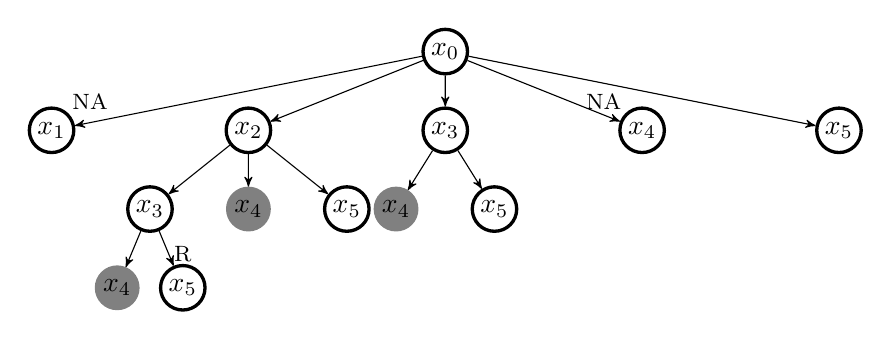
\begin{tikzpicture}[->,>=stealth',level/.style={sibling distance = 2.5cm/#1,
		  level distance = 1cm}] 
		\node [circ] {$x_0$}
		    child{ node [circ] {$x_1$}   
		    node[above right=0.4em] {\footnotesize{NA}}
		    }
		    child{ node [circ] {$x_2$} 
		        child{ node [circ] {$x_3$} 
					child{ node [disc] {$x_4$}}
					child{ node [circ] {$x_5$}
						    node[above=0.6em] {\footnotesize{R}}
					}
		        }
		        child{ node [disc] {$x_4$}}
		        child{ node [circ] {$x_5$}}
			}
			child{ node [circ] {$x_3$}
				child{ node [disc] {$x_4$}}
				child{ node [circ] {$x_5$}}
			}
			child{ node [circ] {$x_4$}
			node[above left=0.4em] {\footnotesize{NA}}
			}
			child{ node [circ] {$x_5$}}
		; 
		\end{tikzpicture}
		\caption{Evaluation of supersets of $x_0$.}
		\label{fig:tree1}
	\end{figure}
	
	Figures~\ref{fig:tree1} (iterations 1--10) and~\ref{fig:tree2} (iterations 11--21) show a tree representation of the algorithm execution for this example. The sequence of evaluated candidates from Table~\ref{tab:cand}, can be used to understand the traversal of the tree representation shown in Figures~\ref{fig:tree1} and~\ref{fig:tree2}. For the following explanation, the nodes which have a gray background should be ignored. Lets begin with the tree shown in Figure~\ref{fig:tree1}, the first evaluation is done over $x_0$. Then, the next level of the tree is created with all the following attributes as children\footnote{The order of attribute is the one that they have in the \textit{SBDM}.}. Each child node is evaluated using the set of all the nodes in the path to its parent as candidate subset. Doing so in the second level of the tree in Figure~\ref{fig:tree1}, $x_1$ and $x_4$ are not accepted (labeled as NA). For each accepted attribute, a new level is constructed with its following accepted attributes as children.
	
	% Second Tree
	\begin{figure}[htb]
		\center
		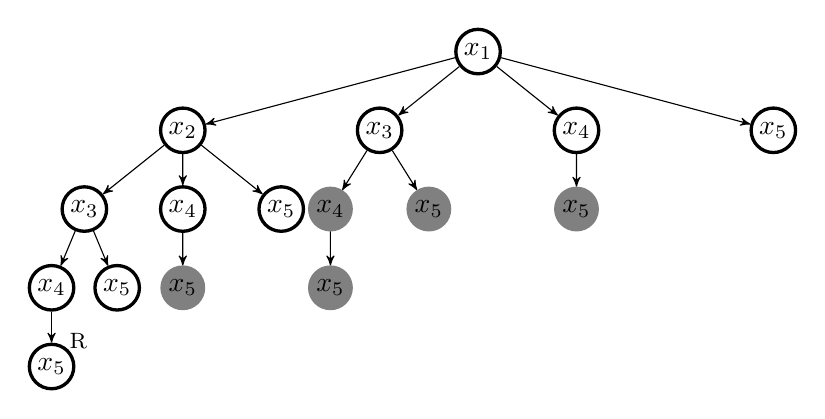
\begin{tikzpicture}[->,>=stealth',level/.style={sibling distance = 2.5cm/#1,
		  level distance = 1cm}] 
		\node [circ] {$x_1$}
		    child{ node [circ] {$x_2$} 
		        child{ node [circ] {$x_3$} 
					child{ node [circ] {$x_4$}
						child{ node [circ] {$x_5$}
							    node[above right=0.3em] {\footnotesize{R}}
						}
					}
					child{ node [circ] {$x_5$}}
		        }
		        child{ node [circ] {$x_4$}
		        	child{ node [disc] {$x_5$}}
		        }
		        child{ node [circ] {$x_5$}}
			}
			child{ node [circ] {$x_3$}
				child{ node [disc] {$x_4$}
					child{ node [disc] {$x_5$}}
				}
				child{ node [disc] {$x_5$}}
			}
			child{ node [circ] {$x_4$}
				child{ node [disc] {$x_5$}}
			}
			child{ node [circ] {$x_5$}}
		; 
		\end{tikzpicture}
		\caption{Evaluation of supersets of $x_1$.}
		\label{fig:tree2}
	\end{figure}
%
\section{Previous Research Work} \label{preliminary}
%
	Our first work in the acceleration of algorithms for computing reduct~\cite{Rodriguez14} consisted in the introduction of a new hardware module into the architecture presented in~\cite{Rojas12}. This new architecture, was capable of identifying the minimal property of typical testors (reducts) in the FPGA device. This modification resulted in a significant runtime reduction, since the platform presented in~\cite{Rojas12} transfers a huge amount of data to the hosting PC and needs a final filtering stage. Then, in~\cite{Rodriguez15}, we presented a hardware-software platform for computing typical testors based on the CT\_EXT algorithm~\cite{Sanchez10}. Even though this platform can process larger basic matrices than previous works, its resource utilization determines the maximum size of the basic matrix that can be solved (this is, indeed, its main limitation). For this reason, we present here an alternative acceleration method, based on algorithm parallelization.
	
	Our most recent work have been directed to the assessment of algorithms' performance regarding some properties of the \textit{SBDM}. We have found some relations that enable the selection, a priori, of the appropriated algorithm for a given dataset. These studies have been submitted for publication at the current time and their results are going to be applied in the evaluation stage of this research proposal. 
%
\section{Concluding Remarks}\label{conclusions}
%

  
% ---- Bibliography ----
%
\bibliographystyle{authordate1}
\bibliography{mybib}

\end{document}